% =========================================================================
\section{Computational Experiments}\label{sec:experiments}
% =========================================================================

The experiments answer five questions, and each subsection opens with its answer.
\begin{enumerate}[label=(Q\arabic*),leftmargin=3em,itemsep=1pt,topsep=3pt]
\item \emph{Is the chain correct?} On every instance small enough to list, the chain visits only feasible states, covers exactly the states its proposal can reach from very different starts, and its empirical law does not depend on the start (Section~\ref{sec:exp-enumeration}).
\item \emph{Is the sampled law stable on instances that cannot be listed?} On grids of $10{,}000$ and $50{,}000$ units and on the London instance, independently started chains agree on every observable to within the noise of a single chain and forget their starts within a few hundred steps (Section~\ref{sec:exp-multistart}).
\item \emph{What does each component of the proposal contribute?} Removing the counting predicate, the residual predicate, the absolute debt window or the local demand target, one at a time, shows which of them the chain cannot run without and which only buy acceptance (Section~\ref{sec:exp-ablation}).
\item \emph{How does the cost of a step scale, and where does the method stop?} The step time grows as about $|V|^{0.55}$ up to $50{,}000$ units; the limit is the team count rather than the graph size, through the supergraph re-partition and the construction of the first plan (Section~\ref{sec:exp-scalability}).
\item \emph{Where does the ensemble sit relative to an optimum?} On the two grids the exact solver can handle, a typical sampled plan is $40$ to $50\%$ above the optimum of a median objective that the sampler never sees, and the same proposal run as an annealer closes most of that distance (Section~\ref{sec:exp-milp}).
\end{enumerate}
Section~\ref{sec:exp-emergency} then applies the sampler to the London Ambulance Service. There is no competing sampler for this state space, so the reference points are exact enumeration, the chain's own components and an exact solver.

% =========================================================================
\subsection{Instances and Protocol}\label{sec:setup}
% =========================================================================

Table~\ref{tab:grids} lists every instance of the paper with the parameters of its runs.

\begin{table}[!htbp]
\centering
\footnotesize\setlength{\tabcolsep}{3.5pt}
\resizebox{\linewidth}{!}{\begin{tabular}{llrrrrcccrl}
\toprule
instance & demand $d_v$ & $|V|$ & $|F^1|$ & $w$ & $k$ & $c^1$ & $c^2$ & $M$ & chains $\times$ steps & used in \\
\midrule
$3\times4$ & $100$ & $12$ & $4$ & $300$ & $4$ & $[1,2]$ & $[2,4]$ & $200/200$ & $3\times200{,}000$ & \ref{sec:exp-enumeration} \\
$4\times4$ & $100$ & $16$ & $5$ & $400$ & $4$ & $[1,2]$ & $[2,4]$ & $200/200$ & $3\times200{,}000$ & \ref{sec:exp-enumeration} \\
$4\times6$ & $100$ & $24$ & $8$ & $400$ & $6$ & $[1,2]$ & $[2,3]$ & $200/200$ & $3\times3{,}000{,}000$ & \ref{sec:exp-enumeration} \\
$4\times4$, mixed & $80$--$120$ & $16$ & $5$ & $400$ & $4$ & $[1,2]$ & $[2,4]$ & $200/200$ & $3\times1{,}000{,}000$ & \ref{sec:exp-enumeration} \\
\midrule
grid\_100 & $U(80,120)$ & $100$ & $8$ & $2{,}000$ & $5$ & $[1,2]$ & $[2,5]$ & $5{,}000/1{,}000$ & $1\times10{,}000$ & \ref{sec:exp-scalability}, \ref{sec:exp-milp} \\
grid\_400 & $U(80,120)$ & $400$ & $15$ & $4{,}000$ & $10$ & $[1,2]$ & $[2,5]$ & $5{,}000/1{,}000$ & $1\times10{,}000$ & \ref{sec:exp-scalability}, \ref{sec:exp-milp} \\
grid\_1000 & $U(80,120)$ & $1{,}000$ & $26$ & $6{,}000$ & $17$ & $[1,2]$ & $[2,5]$ & $5{,}000/1{,}000$ & $1\times10{,}000$ & \ref{sec:exp-ablation}, \ref{sec:exp-scalability} \\
grid\_10000 & $U(80,120)$ & $10{,}000$ & $77$ & $20{,}000$ & $51$ & $[1,2]$ & $[2,5]$ & $5{,}000/1{,}000$ & $4\times30{,}000$ & \ref{sec:exp-multistart}--\ref{sec:exp-scalability} \\
grid\_50000 & $U(80,120)$ & $50{,}000$ & $168$ & $45{,}000$ & $112$ & $[1,2]$ & $[2,5]$ & $5{,}000/1{,}000$ & $4\times30{,}000$ & \ref{sec:exp-multistart}, \ref{sec:exp-scalability} \\
\midrule
London & incidents & $4{,}994$ & $66$ & $10{,}887$ & $97$ & $[1,3]$ & $[2,6]$ & $1{,}000/1{,}000$ & $5\times80{,}000$ & \ref{sec:exp-multistart}, \ref{sec:exp-ablation}, \ref{sec:exp-emergency} \\
\bottomrule
\end{tabular}}
\caption{Instances and run parameters. $k = \lceil d/w\rceil$ is the number of capacity units, $c^1$ and $c^2$ are the capacity ranges of a district and a superdistrict, and $M$ is the retry budget of the tree cut at the base level and at the supergraph. On every instance $\varepsilon^1 = \varepsilon^2 = 0.15$, $\kappa^2_{\min} = 2$ and $F^2 = F^1$, except that on London a level-2 facility must be an open station. The run length is that of the main experiment on the instance; the grids are also run for $10{,}000$ steps in the scaling sweep of Section~\ref{sec:exp-scalability}.}
\label{tab:grids}
\end{table}

\paragraph{Synthetic grids.}
The five grids have i.i.d.\ demands $d_v \sim \mathrm{Uniform}(80,120)$. The workload of a unit is $w = 200\sqrt{|V|}$, rounded to the nearest thousand, so that the number of units $k$ and the mean district size $|V|/k$ both grow as $\sqrt{|V|}$ and neither collapses as the grid grows. The candidate set is sparse, as on London: $\lceil 1.5\,k\rceil$ sites placed uniformly at random, between $8\%$ of the nodes on grid\_100 and $0.3\%$ on grid\_50000. Assumption~\ref{asm:facility-density} therefore fails on every grid by design, and the chain runs on the counting predicate of Section~\ref{sec:capacitated}. Appendix~\ref{app:density} repeats two grids at $1.0$ and $0.7$ sites per unit, the London ratio. The tolerance $0.15$ is above the granularity floor $\varepsilon^1 w \ge d_{\max}$ on every grid and below the bound $2/5$ of Claim~\ref{claim:app-unique}. The level-2 capacity bound $c^2_{\max} = 5$ exceeds the safe range $c \le 3$ of Corollary~\ref{cor:app-invariant}; that range concerns the debt-corrected window of level $1$, and the supergraph recursion carries no debt term and has no closing guarantee (Appendix~\ref{app:debt}). On the grids the level-2 windows are centred at $w$, which differs from $\bar d = d/k$ by $0.9$ to $2.3\%$; the London chains use $\bar d$.

\paragraph{Protocol.}
Every chain uses uniform cut selection and accepts every proposal that closes; a proposal that does not close leaves the state unchanged and is counted. Chains on the large instances start from a zone-wise initial plan that carries exactly $k$ units: rectangular blocks of about $5{,}000$ nodes on the grids and the five operational sectors on London, each cut by the recursive partitioning phase against its own per-unit demand. The first $20\%$ of every chain is discarded.

\paragraph{Diagnostics.}
Agreement between chains is measured on scalar observables: the level-1 access cost $\sum_{D\in\Pc^1}\sum_{v\in D} d_v\,\mathrm{d}(f^1(D),v)$, which is the slowest observable since one superdistrict is re-cut per step, the numbers of districts and superdistricts, and the number of cut edges. For each observable we report the largest Kolmogorov--Smirnov distance between the post-burn-in series of two chains, on every twentieth step. The series are autocorrelated, so the critical values of the two-sample test do not apply, and the reference is the same distance between the two halves of one chain. This reference calibrates the noise of the statistic. It cannot detect a region that all chains miss, which is why Section~\ref{sec:exp-enumeration} checks the support exhaustively where that is possible. \emph{Steps to forget} is the number of steps after which the share of the initial plan's district boundary that is still in place comes within $10\%$ of the share that two independently started plans have in common. Split-$\hat R$ and the effective sample size are reported for the access cost.

\paragraph{Rejections.}
A proposal is rejected for one of four reasons (Section~\ref{sec:feasibility}). At the supergraph, a \emph{tree failure} means that none of the $M$ spanning trees had an admissible pendant subtree although the residual lies inside the window of its remaining capacity, and a \emph{demand failure} means that the residual lies outside that window, so that no tree can close. A re-cut that would leave the selected superdistrict with fewer than $\kappa^2_{\min}$ districts is rejected as \emph{below~$\kappa$}. A \emph{base-level failure} is a level-1 recursion that exhausts its budget. Table~\ref{tab:rejections} in Section~\ref{sec:exp-multistart} reports all four on every instance.

\paragraph{Hardware.}
All chains ran on a single core of a four-core cloud container. The exact solver and the annealing runs of Section~\ref{sec:exp-milp} ran on a laptop with an Apple M3 processor, which is about twice as fast per core. Timings are therefore compared only within one machine. The experiment code, the instances and the stored outputs of every run are in the companion repository~\citep{falcomchain}.

% =========================================================================
\subsection{Correctness on Enumerable Instances}
\label{sec:exp-convergence}\label{sec:exp-enumeration}
% =========================================================================

\emph{Finding.} On four instances whose states can be listed, three chains from very different starts visit only feasible states, cover exactly the set of states that the proposal can reach, and produce the same empirical law to within sampling noise. That law is neither uniform nor the spanning-tree law. With non-uniform demand the reachable set is a proper subset of the states that the balance rule admits.

Section~\ref{sec:convergence-status} explained why no closed-form stationary distribution is available. We therefore validate the chain the way recombination chains are validated in redistricting~\citep{fifield2020essential,cannon2026spanning}: exhaustively where the state space can be listed. On the first three instances of Table~\ref{tab:grids} every unit has demand $100$, so a level-1 district is admissible exactly when it is a connected set of one or two units' worth of nodes that contains a candidate, and the feasible hierarchical states can be listed by exact cover. The $3\times4$ and $4\times4$ grids have one or two superdistricts in every state; the $4\times6$ grid has two or three, so that the supergraph recursion is exercised. Table~\ref{tab:enum} reports the results.

\begin{table}[!htbp]
\centering
\footnotesize\setlength{\tabcolsep}{3.5pt}
\resizebox{\linewidth}{!}{\begin{tabular}{llrrrrrrrrr}
\toprule
 & & \multicolumn{2}{c}{feasible states} & & \multicolumn{3}{c}{TV between chains (noise floor)} & \multicolumn{2}{c}{TV of pooled law to} & \\
\cmidrule(lr){3-4}\cmidrule(lr){6-8}\cmidrule(lr){9-10}
grid & demand & level 1 & joint & unvisited & level 1 & halves & joint & uniform & tree & max/min \\
\midrule
$4\times4$ & $100$ & $435$ & $595$ & 0 & $0.024$ ($0.021$) & $0.033$ ($0.029$) & $0.026$ ($0.022$) & $0.51$ & $0.43$ & $6{,}381$ \\
$4\times6$ & $100$ & $22{,}549$ & $43{,}689$ & 14 (53) & $0.050$ ($0.035$) & $0.069$ ($0.049$) & $0.062$ ($0.047$) & $0.59$ & $0.32$ & $63{,}724$ \\
\midrule
$4\times4$ & $80$--$120$ & $454$ & $614$ & 0 & $0.010$ ($0.009$) & $0.014$ ($0.013$) & $0.012$ ($0.010$) & $0.51$ & $0.43$ & $2{,}807$ \\
\bottomrule
\end{tabular}
}
\caption{Exact enumeration. On the three grids with demand $100$ the feasible states are those that satisfy the rules of Section~\ref{sec:rules}; on the grid with demands $80$ to $120$ they are the states the proposal can reach, computed by closing its move rules, out of $3{,}087$ level-1 states that the balance rule admits. ``Unvisited'' is the number of feasible level-1 states that no chain visited, with the number an independent sample of the same total length from the pooled law would leave unvisited in parentheses. The total-variation (TV) distances are the largest over pairs of chains for the level-1 law and the joint (level-1, level-2) law, and the largest over chains between the two halves of one chain; each is followed in parentheses by its noise floor, the distance expected between two independent samples of the same size from the pooled law. The last three columns describe the pooled level-1 law: its distance to the uniform law and to the spanning-tree law, and the ratio of the largest to the smallest sampled frequency.}
\label{tab:enum}
\end{table}

\paragraph{Soundness and support.}
No chain produced a district without a candidate, a demand outside its window, a superdistrict with fewer than $\kappa^2_{\min}$ districts or a disconnected part. On the two smaller grids every chain visited every level-1 and every joint state. On the $4\times6$ grid the three chains together visited all but $14$ of the $22{,}549$ level-1 states and all but $45$ of the $43{,}689$ joint states, fewer than an independent sample of the same length would miss. Acceptance is $96$ to $97\%$, and almost every rejection is a re-cut below $\kappa$.

\paragraph{Start-independence.}
Every distance between two chains, and between the two halves of one chain, is within a factor of $1.5$ of its noise floor (Table~\ref{tab:enum}). The empirical law is determined by the chain and not by its start, at level 1 and jointly.

\paragraph{What the law is.}
The sampled law is far from uniform, at total-variation distance $0.40$ to $0.59$, and far from the spanning-tree law, at $0.32$ to $0.43$; the most and least frequent states differ in frequency by factors of $262$ to $63{,}724$. Figure~\ref{fig:enumeration} shows its structure on the largest instance. Across capacity mixes the mass lies between the two reference laws: the mixes with two, one and no two-unit districts receive $0.67$, $0.25$ and $0.08$, against $0.54$, $0.40$, $0.06$ under the uniform law and $0.83$, $0.16$, $0.01$ under the spanning-tree law. Within a mix the frequencies follow the spanning-tree weights, the compactness preference that ReCom inherits from cutting random spanning trees, at a distance of $0.28$. On the two smaller grids the mass across mixes is almost uniform instead, so this description is a property of the instance and not of the chain. Given the level-1 plan, the level-2 grouping is close to uniform over the feasible groupings on the $4\times6$ grid (mean distance $0.07$) and far from it on the two smaller grids ($0.45$), where few states admit more than one grouping. On larger instances the law is known only through its support and through the agreement of independently started chains.

\begin{figure}[!htbp]
\centering
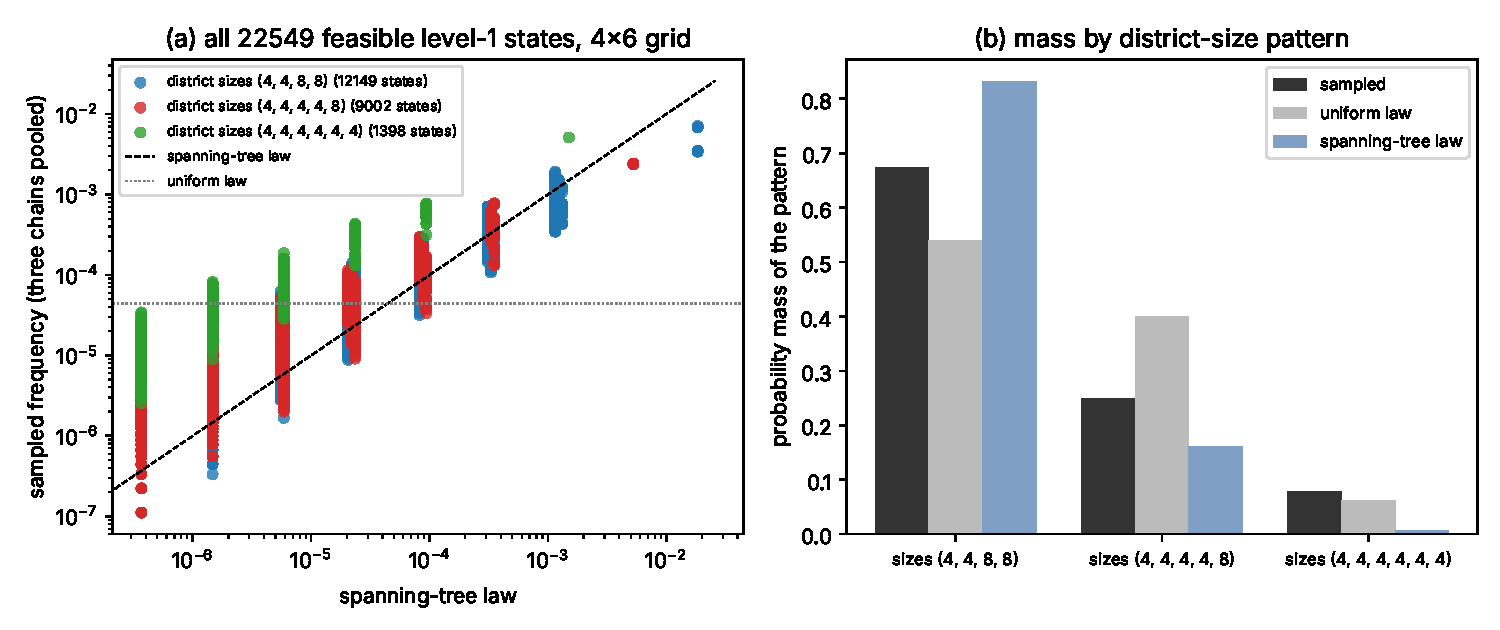
\includegraphics[width=\linewidth]{figures/validation/fig_enumeration_4x6.pdf}
\caption{The sampled level-1 law on the $4\times6$ grid, three chains pooled. Left: sampled frequency of each of the $22{,}549$ feasible states against the spanning-tree law, on logarithmic axes, coloured by district-size pattern; the dotted line is the uniform law. Right: probability mass of each district-size pattern under the sampled, uniform and spanning-tree laws.}
\label{fig:enumeration}
\end{figure}

\paragraph{Non-uniform demand and the reachable set.}
With demand $100$ on every unit, every admissible district has demand exactly $c\,\bar d$, the running debt of the recursion is identically zero, and the three instances above validate the tree cut and the support but not the debt mechanism. The fourth instance of Table~\ref{tab:grids} is the $4\times4$ grid with integer demands between $80$ and $120$ that sum to $4w$. A sampled one-unit district now has four or five nodes and a two-unit district seven to nine, every sampled state has a district off the centre of its window, and the debt is non-zero in every recursion.

On this instance the feasible set has to be defined with more care. The balance rule of Proposition~\ref{prop:effective} is an outer description, and $3{,}087$ level-1 states satisfy it. The proposal cannot produce all of them, because each district is extracted against the debt-corrected window of the recursion at the current debt, which is narrower than the compounded window of the rule. We therefore compute the reachable set independently of the sampler. Starting from the plans that one recursion on the whole graph can produce, we apply every move that the rules of Section~\ref{sec:falcom} allow, that is, every admissible level-2 grouping followed by every sequential extraction of a connected district with a connected complement that is admissible at the current debt under the candidate and counting predicates, and we close the set under these moves. No spanning tree is drawn, so the result does not depend on the retry budget. The closure has $454$ level-1 states and $614$ joint states and is a single communicating class. Two further states can be reached only through a district whose demand lies exactly on the edge of its window, a tie that floating-point rounding decides in the implementation, and we exclude them.

The three chains start from the first, middle and last state of the outer set, none of which the proposal can itself produce. Each chain visits all $454$ reachable level-1 states and all $614$ joint states, and no chain visits any other state (Table~\ref{tab:enum}, last row). Their laws agree to within the noise floor, and the sampled law is again far from uniform on its support. On an instance that exercises the debt mechanism, the support of the chain is thus exactly the reachable set of its proposal and that set is irreducible. It is also a proper subset, $15\%$, of the states that the balance rule admits: the loads of sampled districts lie between $0.89$ and $1.15$ of their capacity, against $0.73$ to $1.32$ under the rule. Proposition~\ref{prop:effective} is a guarantee that every sampled state satisfies, not a description of the support, and this instance answers in the negative the question, left open in Section~\ref{sec:rules}, of whether every state that satisfies the rule is reachable.

% =========================================================================
\subsection{Stability on Large Instances}
\label{sec:exp-multistart}
% =========================================================================

\emph{Finding.} On grid\_10000, grid\_50000 and London, independently started chains differ from each other no more than one chain differs from itself on ten of twelve observables, slightly more on the other two, and every chain forgets its start within $800$ steps, a small fraction of its length.

Where enumeration is impossible we run four chains from independently drawn zone-wise plans and compare them with the diagnostics of Section~\ref{sec:setup}. The London instance is described in Section~\ref{sec:exp-emergency}; its chains are included here so that all three instances are read against the same table. On London the four chains share the sector-wise construction, so a fifth chain was started from a structurally different plan, built inside the $21$ real Groups with the three single-station Groups merged into their neighbours ($18$ zones instead of five). Table~\ref{tab:multistart} and Figure~\ref{fig:forgetting} report the diagnostics.

\begin{table}[!htbp]
\centering
\footnotesize\setlength{\tabcolsep}{3.5pt}
\resizebox{\linewidth}{!}{\begin{tabular}{llrrrrrrrr}
\toprule
 & & & \multicolumn{4}{c}{Kolmogorov--Smirnov distance} & & & \\
\cmidrule(lr){4-7}
instance & & acceptance & access cost & $|\Pc^1|$ & $|\Pc^2|$ & cut edges & steps to forget & $\hat R$ & ESS \\
\midrule
grid\_10000 & between chains & 89.4--89.5\% & $0.042$ & $0.044$ & $0.042$ & $0.077$ & $180$--$360$ & $1.001$ & $1{,}740$ \\
 & within a chain & & $0.053$--$0.080$ & $0.012$--$0.025$ & $0.029$--$0.069$ & $0.086$--$0.136$ & & & \\
grid\_50000 & between chains & 85.5--86.4\% & $0.090$ & $0.052$ & $0.057$ & $0.095$ & $540$--$780$ & $1.005$ & $647$ \\
 & within a chain & & $0.045$--$0.075$ & $0.027$--$0.075$ & $0.048$--$0.096$ & $0.089$--$0.147$ & & & \\
London & between chains & 67.7--68.0\% & $0.078$ & $0.037$ & $0.020$ & $0.070$ & $400$--$520$ & $1.003$ & $1{,}760$ \\
 & within a chain & & $0.022$--$0.088$ & $0.021$--$0.067$ & $0.011$--$0.039$ & $0.022$--$0.083$ & & & \\
London, fifth chain & to the four chains & 68.4\% & $0.072$ & $0.033$ & $0.018$ & $0.081$ & $680$ & $1.002$ & $470$ \\
\bottomrule
\end{tabular}
}
\caption{Multi-start agreement. ``Between chains'' is the largest pairwise Kolmogorov--Smirnov distance among four chains after burn-in; ``within a chain'' is the range over chains of the same distance between the two halves of one chain, the noise reference. For the fifth London chain the distances are the largest to any of the four sector-start chains. $\hat R$ and the effective sample size (summed over the chains) refer to the access cost. Grid chains have $30{,}000$ steps and London chains $80{,}000$; the access cost and $|\Pc^1|$ are read on every twentieth step, and $|\Pc^2|$ and the cut edges on the stored plans of the grids (every $60$th step).}
\label{tab:multistart}
\end{table}

\begin{figure}[!htbp]
\centering
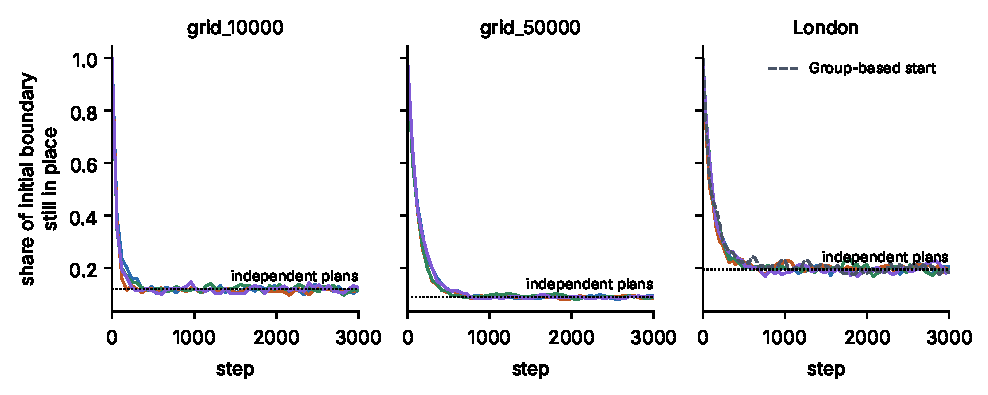
\includegraphics[width=\linewidth]{figures/sec7/fig_forgetting.pdf}
\caption{Forgetting the start: the share of the initial plan's district boundary that is still a district boundary, for each chain, over the first $3{,}000$ steps. The dotted line is the share that two independently started plans have in common. The dashed curve on London is the chain started from the Group-based plan.}
\label{fig:forgetting}
\end{figure}

\paragraph{Agreement.}
On ten of the twelve instance and observable pairs the chains differ from each other no more than one chain differs from itself. The exceptions are the number of districts on grid\_10000 ($0.044$ against a within-chain maximum of $0.025$) and the access cost on grid\_50000 ($0.090$ against $0.075$). At the effective sample sizes of Table~\ref{tab:multistart} a difference in distribution of this size is at the limit of what the runs can detect, and split-$\hat R$ is at most $1.005$. The fifth London chain is as close to the four sector-start chains as they are to each other: its distances lie inside the within-chain range on every observable, its mean energy, number of open stations and adjusted Rand index against the real Groups lie within the ranges of the four, and its station open frequencies differ from the pooled four by about as much as one of the four does, at most $0.05$ against $0.045$ (Appendix~\ref{app:london-extra}). A start with a different level-2 structure thus reaches the same law.

\paragraph{Forgetting.}
The chains lose memory of their starts within $180$ to $780$ steps, for plans of $38$ to $85$ districts, after which the share of the initial boundary still in place stays at the independent-plan value (Figure~\ref{fig:forgetting}). The burn-in of $20\%$ is therefore conservative by more than an order of magnitude. This is the locality argument of Section~\ref{sec:convergence-status} at work: every level-2 boundary is redrawn at every step and one superdistrict is re-cut, so the number of steps needed scales with the number of superdistricts.

\paragraph{Rejections.}
Table~\ref{tab:rejections} splits the rejected proposals by cause. Rejections are a supergraph phenomenon on every instance. Base-level failures stay below five per $10{,}000$ proposals, which is the price of a candidate set with $1.5$ sites per unit, or $0.7$ on London, once the counting predicate is in place. Supergraph tree failures grow with the number of supernodes, from none on grid\_100 to $7.5\%$ on grid\_50000, and reach $26\%$ on London, where a superdistrict holds two to six units in stations of one to three and the windows are correspondingly harder to hit with a pendant subtree. Demand failures stay below $2\%$. In the multi-start runs on grid\_50000, $14$ of $120{,}000$ proposals were in addition rejected by a numerical guard that re-checks the per-unit balance~\eqref{eq:per-team-window} of a returned cut; in exact arithmetic the guard cannot fire, and it did not on any other instance. Every rejection is a repeated state, not an error; the holding times of rejected proposals enter the sampled law, and Appendix~\ref{app:london-extra} quantifies that effect on London, where it is largest.

\begin{table}[!htbp]
\centering
\small
\begin{tabular}{lrrrrrr}
\toprule
 & & & \multicolumn{2}{c}{supergraph recursion} & superdistrict & base-level \\
\cmidrule(lr){4-5}
instance & proposals & accepted & tree failure & demand failure & below $\kappa^2_{\min}$ & failures per $10^4$ \\
\midrule
grid\_100 & $9{,}999$ & 94.7\% & 0.0\% & 0.0\% & 5.3\% & $0.0$ \\
grid\_400 & $9{,}999$ & 92.5\% & 0.3\% & 0.3\% & 7.0\% & $0.0$ \\
grid\_1000 & $9{,}999$ & 91.6\% & 1.4\% & 1.1\% & 5.9\% & $2.0$ \\
grid\_10000 & $9{,}999$ & 89.8\% & 3.5\% & 1.8\% & 4.9\% & $2.0$ \\
grid\_50000 & $9{,}999$ & 86.4\% & 7.5\% & 1.7\% & 4.3\% & $4.0$ \\
London & $319{,}996$ & 67.8\% & 25.8\% & 0.3\% & 6.0\% & $1.9$ \\
\bottomrule
\end{tabular}

\caption{Rejected proposals by cause, as shares of all proposals: the scaling sweep on the grids (one chain of $10{,}000$ steps each) and the four London chains pooled. The four causes are defined in Section~\ref{sec:setup}.}
\label{tab:rejections}
\end{table}

% =========================================================================
\subsection{What Each Component Contributes}\label{sec:exp-ablation}
% =========================================================================

\emph{Finding.} Each of the four components of the proposal is needed. Removing the counting predicate, the absolute debt window or the local demand target raises base-level failures from two in ten thousand proposals to between $9\%$ and $46\%$ of them, and removing the residual predicate raises supergraph failures from $3$--$5\%$ to $36$--$40\%$ on the grids and from $27\%$ to $57\%$ on London. The retry budget, in contrast, has no detectable effect on the readouts between $200$ and $5{,}000$ trees.

No other sampler exists for this state space, so we measure the sampler against itself. Each variant switches off or replaces exactly one component and leaves everything else at the calibration of the instance. The initial plan is always built with the full method, so that a variant measures what the component contributes inside the chain. We run one chain per variant on grid\_1000, grid\_10000 and London, for $10{,}000$ steps on the first and $5{,}000$ on the other two, or for as many proposals as fit in fifteen minutes, since a variant can make a proposal a hundred times slower. Table~\ref{tab:ablation} reports the results.

\begin{table}[!htbp]
\centering
\small\setlength{\tabcolsep}{4pt}
\resizebox{\linewidth}{!}{\begin{tabular}{lrrrrrrrrr}
\toprule
 & \multicolumn{3}{c}{grid\_1000} & \multicolumn{3}{c}{grid\_10000} & \multicolumn{3}{c}{London} \\
\cmidrule(lr){2-4}\cmidrule(lr){5-7}\cmidrule(lr){8-10}
variant & accepted & base & supergr. & accepted & base & supergr. & accepted & base & supergr. \\
\midrule
FalCom (all components) & 91.6\% & 0.02\% & 2.5\% & 89.6\% & 0.02\% & 5.3\% & 66.5\% & 0.02\% & 27.2\% \\
\midrule
no counting predicate & 82.3\% & 9.9\% & 2.5\% & 80.6\% & 8.7\% & 5.3\% & 53.3\% & 11.9\% & 28.8\% \\
no residual predicate & 60.1\% & 0.03\% & 36.2\% & 56.8\% & 0.02\% & 40.0\% & 39.6\% & 0.02\% & 57.0\% \\
capacity-scaled debt window & 67.4\% & 18.1\% & 10.9\% & 63.8\% & 14.2\% & 19.1\% & 42.4\% & 17.5\% & 35.5\% \\
global demand target at level 1 & 59.2\% & 34.5\% & 0.6\% & 48.4\% & 45.6\% & 0.5\% & 32.5\% & 38.5\% & 23.9\% \\
\bottomrule
\end{tabular}
}
\caption{Component ablations: one chain per variant and instance. ``Accepted'' is the share of proposals that close. ``Base'' and ``supergr.''\ are the shares of proposals rejected because the level-1 recursion or the supergraph recursion exhausted its retry budget; the remaining rejections are re-cuts below $\kappa$. Variants that reached the fifteen-minute cap made fewer proposals than the full method: without the counting predicate, with the scaled window and with the global target, $2{,}194$, $1{,}262$ and $490$ on grid\_1000 and $995$, $755$ and $182$ on grid\_10000, and $2{,}405$ with the global target on London.}
\label{tab:ablation}
\end{table}

\paragraph{Counting predicate.}
Without the counting predicate a level-1 cut only requires a candidate on each side, and the greedy extraction can leave a residual with fewer candidates than the districts it still has to form. Base-level failures then rise from $0.02\%$ of proposals to $9$--$10\%$ on the grids and $12\%$ on London, and each failure spends the whole retry budget, so that a proposal takes $18$ to $28$ times as long on the grids. Inside a chain the damage is bounded, because a re-cut concerns one superdistrict of a few districts. When a plan is built from nothing it is not: on a $20\times20$ grid with twelve candidates for ten districts the recursion without the predicate did not produce an initial plan in $5{,}000$ tree draws, and with it the plan closes at the first attempt (Section~\ref{sec:feasibility}).

\paragraph{Residual predicate.}
The residual predicate is the level-2 analogue: it admits a supergraph extraction only if the supernodes left behind can still be grouped. Without it the supergraph recursion strands a final supernode, and supergraph failures rise from $2.5\%$ and $5\%$ of proposals to $36\%$ and $40\%$ on the two grids and from $27\%$ to $57\%$ on London, where acceptance falls from $66\%$ to $40\%$. Both predicates are necessary conditions for a recursion to close, so neither changes the set of reachable states; they remove proposals that were certain to fail.

\paragraph{Absolute debt window.}
The debt-corrected window of Section~\ref{sec:recursive} holds a district of capacity $c$ to the same absolute half-width as a one-unit district. The natural alternative scales the window with $c$ (Remark~\ref{rem:app-scaled}). It admits more cuts for $c \ge 2$, but the debt can then leave the envelope in which the remaining windows are non-empty, and $14\%$ to $18\%$ of proposals fail at the base level on the three instances. The less balanced districts also make the supergraph harder to re-partition: its failures rise on every instance, and on London its demand failures go from $0.5\%$ to $10\%$. This is the practical content of Corollary~\ref{cor:app-invariant}.

\paragraph{Local demand target.}
At the lower level the recursion is centred on the per-unit demand of the superdistrict being re-cut, not on the global one, so that it starts with zero debt (Lemma~\ref{lem:app-telescoping}). With the global target the recursion starts in debt whenever the selected superdistrict is denser or sparser than average, and $35\%$ to $46\%$ of proposals fail at the base level, the largest effect of the four; a proposal then takes up to a hundred times as long.

\paragraph{Retry budget.}
The retry budget $M$ enters the proposal kernel, and so in principle the sampled law (Section~\ref{sec:convergence-status}). Table~\ref{tab:budget} varies it from $200$ to $5{,}000$ trees at both levels. Acceptance changes by about one point. The mean access cost stays within $0.4\%$ of the reference and the mean number of districts varies by at most $0.6$ across budgets, with no trend in $M$, and the Kolmogorov--Smirnov distances of the varied budgets ($0.06$ to $0.14$ on grid\_10000 and London, where each short run is compared with the long chains of Section~\ref{sec:exp-multistart}) are of the same size as those of the default runs. The runs are short, so a shift in distribution below about $0.1$ would not be detected; within that resolution the readouts do not depend on the budget.

\begin{table}[!htbp]
\centering
\small
\begin{tabular}{lrrrrrrr}
\toprule
 & \multicolumn{2}{c}{retry budget $M$} & & \multicolumn{2}{c}{access cost} & \multicolumn{2}{c}{$|\Pc^1|$} \\
\cmidrule(lr){2-3}\cmidrule(lr){5-6}\cmidrule(lr){7-8}
instance & base & supergraph & accepted & mean (rel.) & KS & mean & KS \\
\midrule
grid\_1000 & $200$ & $200$ & 91.8--92.4\% & $1.002$ & $0.046$ & $12.7$ & $0.044$ \\
grid\_1000 & $1{,}000$ & $1{,}000$ & 91.8--92.0\% & $0.999$ & $0.027$ & $12.6$ & $0.009$ \\
grid\_1000 & $5{,}000$ & $1{,}000$ & 91.6--92.0\% & $1.000$ & $(0.050)$ & $12.7$ & $(0.030)$ \\
grid\_1000 & $5{,}000$ & $5{,}000$ & 91.3--92.1\% & $1.001$ & $0.046$ & $12.7$ & $0.046$ \\
\midrule
grid\_10000 & $200$ & $200$ & 89.2--89.5\% & $0.999$ & $0.064$ & $38.6$ & $0.073$ \\
grid\_10000 & $1{,}000$ & $1{,}000$ & 88.4--89.7\% & $0.998$ & $0.144$ & $38.2$ & $0.100$ \\
grid\_10000 & $5{,}000$ & $1{,}000$ & 89.6--89.7\% & $0.996$ & $(0.144)$ & $38.2$ & $(0.061)$ \\
grid\_10000 & $5{,}000$ & $5{,}000$ & 89.2--89.7\% & $0.999$ & $0.074$ & $38.6$ & $0.070$ \\
\midrule
London & $200$ & $200$ & 65.4--66.4\% & $1.001$ & $0.078$ & $52.1$ & $0.129$ \\
London & $1{,}000$ & $1{,}000$ & 66.5--69.4\% & $0.996$ & $(0.143)$ & $52.7$ & $(0.115)$ \\
London & $5{,}000$ & $5{,}000$ & 66.3--67.1\% & $1.003$ & $0.097$ & $52.2$ & $0.084$ \\
\bottomrule
\end{tabular}

\caption{Sensitivity to the retry budget $M$, two seeds per setting. Acceptance is the range over the seeds. For grid\_10000 and London the Kolmogorov--Smirnov distances are from each run to the long chains of Table~\ref{tab:multistart} (largest over the two seeds), and the mean access cost is relative to those chains; for grid\_1000 they are to the pooled default runs. Values in parentheses are the default setting, which gives the noise of the comparison.}
\label{tab:budget}
\end{table}

\paragraph{Chain against independent draws, and candidate density.}
Two further comparisons are reported elsewhere. A plan can also be drawn by one recursion on the whole graph, independently of any previous plan; on grid\_50000 such a recursion did not close within half an hour, and on London it rarely closes within its budget, which is why FalCom is a chain that re-cuts one superdistrict per step (Section~\ref{sec:convergence-status}). Appendix~\ref{app:density} varies the candidate density from $1.5$ to $0.7$ sites per unit: the chain keeps running at every density, and what the density affects is the construction of the first plan.



% =========================================================================
\subsection{Scalability}\label{sec:exp-scalability}
% =========================================================================

\emph{Finding.} The time of an accepted step grows as about $|V|^{0.55}$ from $100$ to $50{,}000$ units, because a step re-cuts one superdistrict and not the graph. The method is limited by the number of units $k$, not by $|V|$: beyond a few hundred units the supergraph re-partition dominates the step and the first plan becomes hard to build.

Contribution~(iii) of Section~\ref{sec:intro} claims that FalCom runs on graphs with up to $50{,}000$ basic units. A step re-cuts one superdistrict at level $1$ and re-partitions the supergraph at level $2$, so its cost has a local part, set by the merged subgraph $H$, and a global part, set by the number of districts. Two sweeps separate them.

\paragraph{Growing graph.}
We run one chain of $10{,}000$ steps on each of the five grids and record the wall-clock time of every proposal and its split between the two levels (Table~\ref{tab:scalability}). Over a $500$-fold range of $|V|$, in which $k$ grows from $5$ to $112$, the median time of an accepted step rises from $3.6$ to $106$\,ms, a factor of $30$, and the mean time per proposal including rejected ones by a factor of $41$, while the share $|H|/|V|$ of the graph that a step touches falls from $0.89$ to $0.031$. The step time grows faster than $|H|$, which rises by a factor of $18$; the difference is the supergraph re-partition, $5\%$ of an accepted step on grid\_100 and $19\%$ on grid\_50000. A rejected proposal spends its whole retry budget, which is why the mean over all proposals lies above the median of the accepted ones. Ten thousand proposals take $28$ minutes on grid\_50000.

\begin{table}[!htbp]
\centering
\footnotesize\setlength{\tabcolsep}{4pt}
\resizebox{\linewidth}{!}{\begin{tabular}{rrrrrrrrrr}
\toprule
$|V|$ & $k$ & $|\Pc^1|$ & mean $|H|$ & $|H|/|V|$ & median step & mean proposal & $95$th pct & supergraph share & $10^4$ proposals \\
\midrule
$100$ & $5$ & $4$ & $89$ & $0.889$ & $3.6$\,ms & $4$\,ms & $8$\,ms & 5\% & $0.7$\,min \\
$400$ & $10$ & $7$ & $143$ & $0.356$ & $5.5$\,ms & $8$\,ms & $15$\,ms & 7\% & $1.3$\,min \\
$1{,}000$ & $17$ & $13$ & $212$ & $0.212$ & $9.3$\,ms & $16$\,ms & $24$\,ms & 9\% & $2.6$\,min \\
$10{,}000$ & $51$ & $38$ & $694$ & $0.069$ & $36.8$\,ms & $56$\,ms & $96$\,ms & 13\% & $9.3$\,min \\
$50{,}000$ & $112$ & $85$ & $1{,}566$ & $0.031$ & $106.5$\,ms & $167$\,ms & $248$\,ms & 19\% & $27.9$\,min \\
\bottomrule
\end{tabular}
}
\caption{Per-step cost on the five grids, one chain of $10{,}000$ steps each. $|\Pc^1|$ is the median number of districts and $|H|$ the number of nodes of the superdistrict that a step re-cuts. The median and the $95$th percentile are over accepted steps; ``mean proposal'' includes rejected ones. ``Supergraph share'' is the share of the time of accepted steps spent re-partitioning the supergraph.}
\label{tab:scalability}
\end{table}

\paragraph{Fixed graph, growing team count.}
With $w \propto \sqrt{|V|}$ the number of units and the district size grow together. To separate them we rebuild grid\_10000 with smaller $w$, at the same $1.5$ candidate sites per unit, and run two seeds of $3{,}000$ steps each (Table~\ref{tab:fixed}). Doubling the number of units from $51$ to $101$ halves $|H|$ and leaves the step time almost unchanged, but the supergraph re-partition now takes about half of it. Doubling again to $201$ makes the supergraph re-partition $84$ to $88\%$ of a step, raises the rejection rate to $21$ to $24\%$, and the zone-wise initial plan needs up to eleven minutes. At $401$ units the initial plan, built in two zones of about $200$ units each, did not close in twelve attempts.

\begin{table}[!htbp]
\centering
\footnotesize\setlength{\tabcolsep}{4pt}
\begin{tabular}{rrrrrrrrr}
\toprule
$w$ & $k$ & $|F^1|$ & $|\Pc^1|$ & initial plan & median step & mean $|H|$ & supergraph share & rejected \\
\midrule
$20{,}000$ & $51$ & $77$ & $38$ & $2$\,s & $37$\,ms & $694$ & 13\% & 10\% \\
$10{,}000$ & $101$ & $152$ & $75$ & $4$--$343$\,s & $30$\,ms & $351$ & 46--51\% & 12--14\% \\
$5{,}000$ & $201$ & $302$ & $148$--$149$ & $49$--$689$\,s & $74$--$78$\,ms & $177$ & 84--88\% & 21--24\% \\
$2{,}500$ & $401$ & $602$ & \multicolumn{6}{l}{initial plan not built in twelve attempts ($19$\,min)} \\
\bottomrule
\end{tabular}

\caption{The $10{,}000$-node grid at a growing number of units $k$, two seeds of $3{,}000$ steps each (one chain of $10{,}000$ steps for $k=51$); ranges are over the seeds. ``Initial plan'' is the time of the zone-wise construction of the first plan.}
\label{tab:fixed}
\end{table}

\paragraph{Working regime.}
On one core the sampler handles graphs of $50{,}000$ units at about a tenth of a second per step, with superdistricts of a few hundred to a few thousand nodes. Its working regime in the number of units is up to a few hundred: the supergraph is re-partitioned from scratch at every step, at a cost that grows with the number of districts, and a plan built from nothing must extract every district in one recursion. Both limits concern the greedy supergraph recursion and the initial plan, not the level-1 move, and Section~\ref{sec:limitations} returns to them.

% =========================================================================
\subsection{The Ensemble Relative to an Exact Optimum}\label{sec:exp-milp}
% =========================================================================

\emph{Finding.} On the two grids that the exact solver can handle, the sampled plans lie $17$ to $65\%$ above the optimum of a median objective, with a typical plan at $43$ to $47\%$; chains agree on this distribution to $0.3\%$. The same proposal run as an annealer comes within $0.9\%$ and $7.5\%$ of the optimum, so the distance is a property of sampling without an objective and not of the moves.

The sampler has no objective. To place its ensemble on an absolute scale we solve the mixed-integer model of Section~\ref{sec:model} exactly on grid\_100 and grid\_400 with the \emph{disaggregated hierarchical median}, the sum of the demand-weighted distances of every unit to its level-1 and to its level-2 facility, in the spirit of the $p$--$q$ median of \citet{serra1993pq}:
\begin{equation}\label{eq:milp-median}
  \min \quad \sum_{\ell \in L} \sum_{i \in V^1} \sum_{j \in F^\ell} d_i \, \mathrm{d}(i, j) \, x^\ell_{ij},
\end{equation}
where $\mathrm{d}(i,j)$ is the Manhattan distance on grid coordinates. The level-1 term involves only $x^1$ and the level-2 term only $x^2$, so each facility sits at the demand-weighted $1$-median of the units it serves, which is the facility rule of Section~\ref{sec:facility}. We then evaluate~\eqref{eq:milp-median} on every state of four sampling chains of $20{,}000$ steps on each grid.

\paragraph{Exact solutions.}
The program is solved with Gurobi~13.0 on four threads, with the flow-based contiguity constraints of Appendix~\ref{app:shir} at level $1$, to a proven optimum (gap $10^{-6}$). The superdistricts of every optimum are connected, so each is also an optimum of the two-level model (Appendix~\ref{app:shir}). The solve takes one second on grid\_100 and $830$ seconds on grid\_400, with $15$ candidate sites for $10$ units. Without any contiguity constraint the optimum is the same on grid\_100 and $0.007\%$ lower on grid\_400, where it splits one district in two: a median objective favours contiguous districts but does not guarantee them.

\begin{table}[!htbp]
\centering
\small
\begin{tabular}{lrrrrrrr}
\toprule
 & & \multicolumn{3}{c}{exact optimum} & \multicolumn{2}{c}{sampled ensemble / optimum} & annealed \\
\cmidrule(lr){3-5}\cmidrule(lr){6-7}
instance & sites / units & objective & time & no contiguity & median & $5$--$95\%$ & / optimum \\
\midrule
grid\_100 & $8$ / $5$ & $61{,}884$ & $1$\,s & $61{,}884$ & $1.43$ & $1.17$--$1.55$ & $1.009$ \\
grid\_400 & $15$ / $10$ & $352{,}810$ & $830$\,s & $352{,}785$ & $1.47$ & $1.33$--$1.65$ & $1.075$ \\
\bottomrule
\end{tabular}

\caption{The sampled ensemble against the exact optimum of objective~\eqref{eq:milp-median}. The ensemble columns are quantiles of the objective over the post-burn-in states of four chains of $20{,}000$ steps, relative to the optimum. ``Annealed'' is the best state of eight annealing runs of $10{,}000$ steps with the same proposal.}
\label{tab:milp}
\end{table}

\begin{figure}[!htbp]
\centering
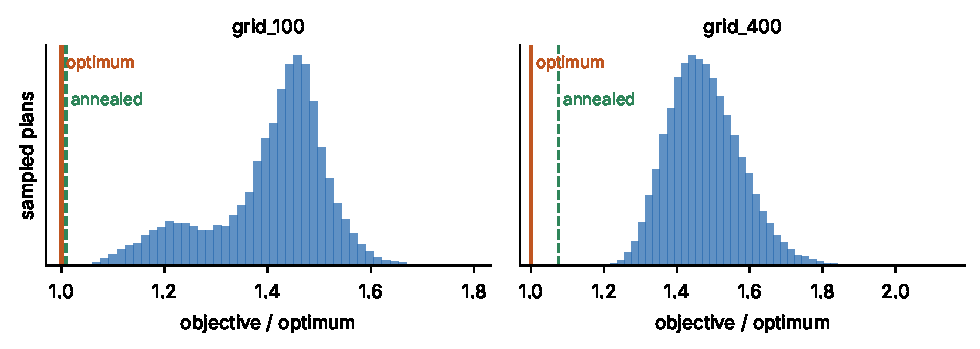
\includegraphics[width=0.9\linewidth]{figures/sec7/fig_placement.pdf}
\caption{Objective~\eqref{eq:milp-median} of the sampled plans relative to the exact optimum, four chains pooled. The solid line is the optimum and the dashed line the best annealed state.}
\label{fig:placement}
\end{figure}

\paragraph{Placement.}
Table~\ref{tab:milp} and Figure~\ref{fig:placement} place the ensemble. No sampled plan on grid\_400 is within $15\%$ of the optimum, and fewer than one in a hundred on grid\_100 is within $10\%$. This is what a sample of the feasible set should look like when it is drawn without regard to the objective: the optimum is an extreme point of a distribution whose bulk is far from it. The mean of the objective differs between chains by at most $0.3\%$, so the placement is a stable property of the sampled law. For a planner the ensemble therefore answers a different question from the solver. It shows how much access cost a balanced, contiguous plan gives up when it is not chosen for access cost, which Section~\ref{sec:exp-emergency} uses on London, and it takes seconds per thousand plans where a proven optimum on $400$ units takes a quarter of an hour.

\paragraph{The proposal as an annealer.}
To check that the distance is not a limitation of the moves, we run the chain with objective~\eqref{eq:milp-median} as an energy: at step $t$ of $T$ an improving proposal is accepted and a worsening one with probability $\exp(-\beta_t\,\Delta E/\sigma)$, with $\beta_t = t/T$ and $\sigma$ the initial energy per unit. The best of eight runs of $T = 10{,}000$ steps is $0.9\%$ above the optimum on grid\_100 and $7.5\%$ on grid\_400 ($4.1\%$ at $T = 200{,}000$), with the same capacity mix and the same open level-2 facilities as the optimum, and one run takes $15$ and $27$ seconds. We use this mode only as a tool: it shows that the moves reach the neighbourhood of the optimum, and Section~\ref{sec:exp-emergency} uses it to tighten a bound. It is a crude annealer and the paper makes no claim for it as an optimizer.

\paragraph{Scope.}
The two feasible sets are not identical. The program uses the windows of constraint~\eqref{cons:balance} at $\varepsilon = 0.15$ around $w$, while a sampled state satisfies the hierarchical rule of Proposition~\ref{prop:effective}; the optimum satisfies both, but some sampled states have districts between $0.83$ and $1.23$ units of $w$ and are not feasible for the program. The comparison is one of objective values, not of optima over one set. The grids have near-uniform demand, on which the optimum uses single-unit districts only. On a variant of grid\_400 with two demand peaks of $1.4\,w$ the optimum uses two-unit districts around the peaks ($1{,}455$ seconds), but the peaks exceed the granularity floor of Section~\ref{sec:capacitated} by an order of magnitude and the sampler cannot build an initial plan at this tolerance; such an instance needs a larger capacity unit, as in the London calibration.
